% AUTO-GENERATED by scripts/11_supplementary_analyses.py - do not edit by hand.

\begin{figure}[htbp]
\centering
\begin{minipage}{0.74\textwidth}\centering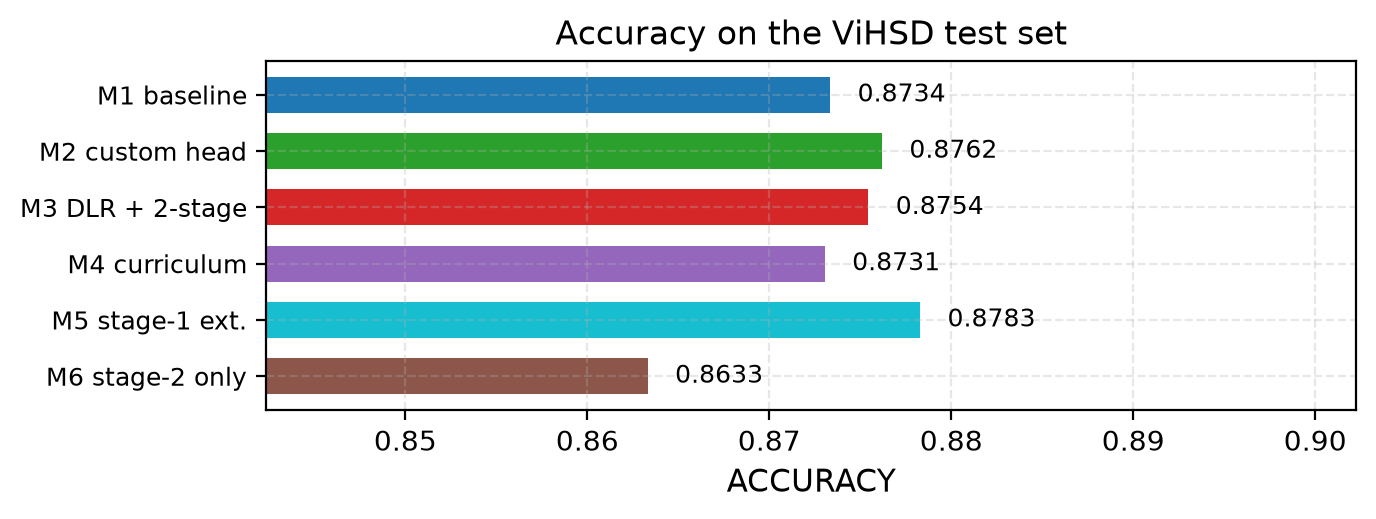
\includegraphics[width=\linewidth]{figures/comparison/accuracy_all_models.png}\caption{\label{fig:supp-acc}Test accuracy for all six systems with 95\% bootstrap confidence intervals.  The highest accuracy belongs to \model{M5}, which does not have the best macro-F1.}\end{minipage}
\end{figure}

\begin{figure}[htbp]
\centering
\begin{minipage}{0.74\textwidth}\centering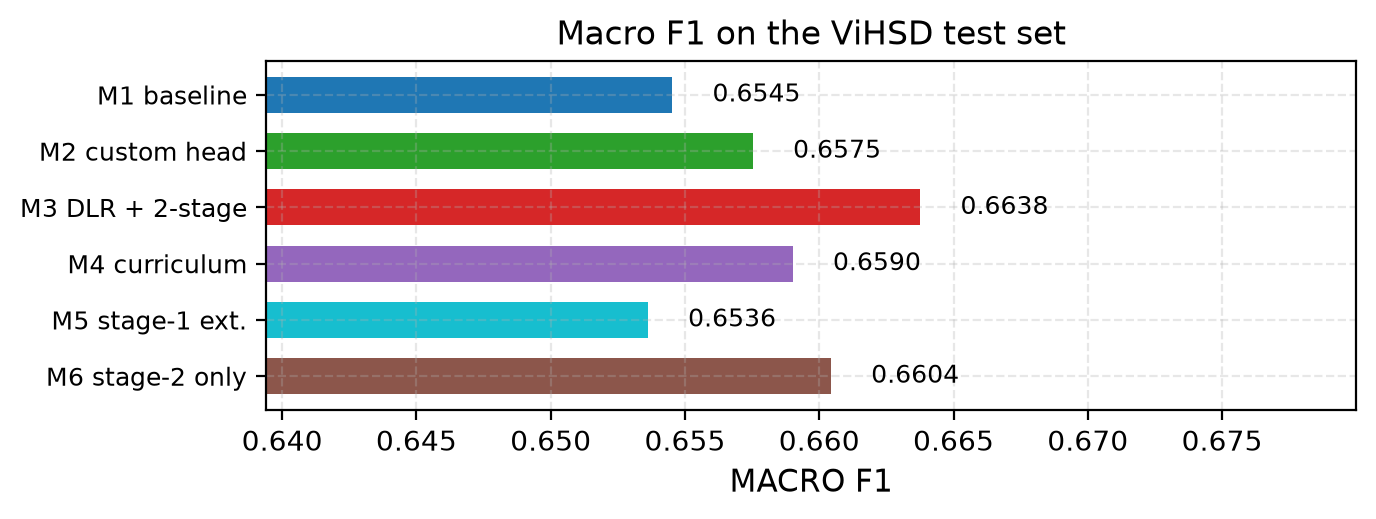
\includegraphics[width=\linewidth]{figures/comparison/macro_f1_all_models.png}\caption{\label{fig:supp-macro-f1}Test macro-F1 (mean of the three class F1 scores) for all six systems.  The six systems sit in a narrow band, which is why no pairwise macro-F1 difference is significant.}\end{minipage}
\end{figure}

\begin{figure}[htbp]
\centering
\begin{minipage}{0.74\textwidth}\centering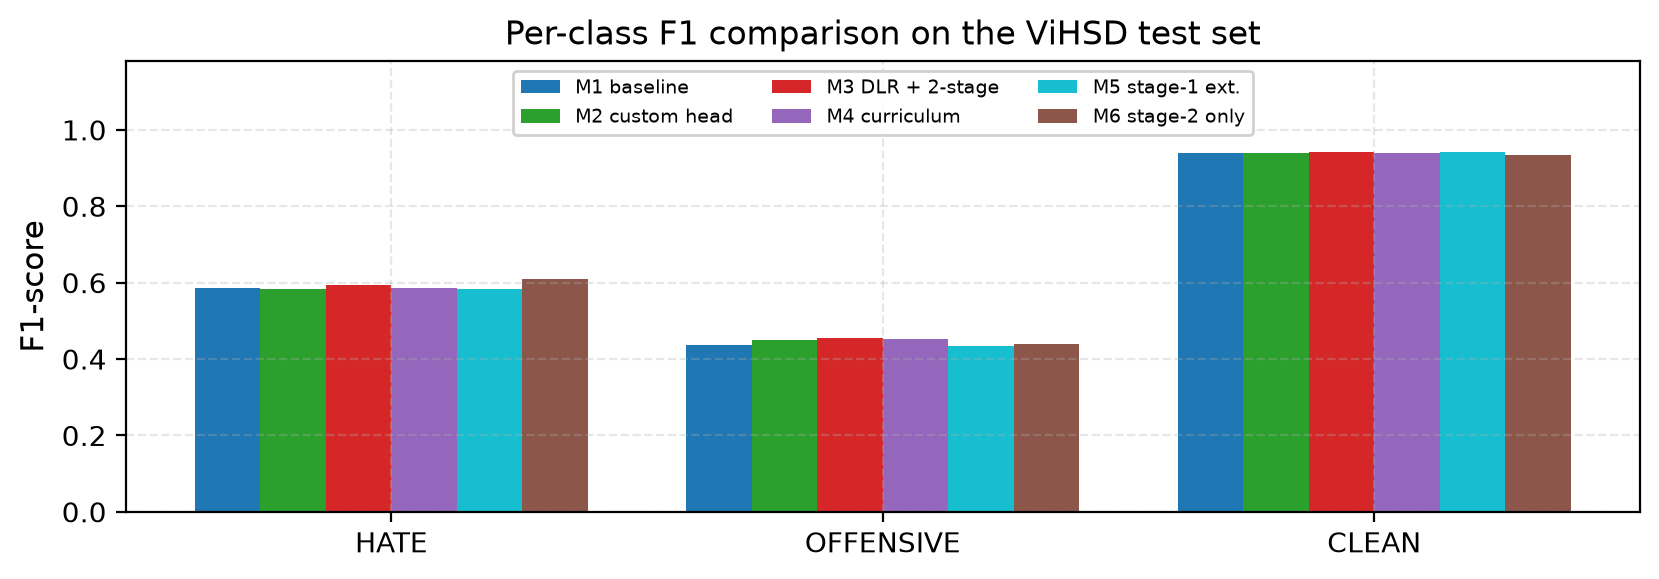
\includegraphics[width=\linewidth]{figures/comparison/per_class_f1_all_models.png}\caption{\label{fig:supp-per-class-f1}Per-class F1 for HATE, OFFENSIVE and CLEAN, grouped by system.  The minority classes (HATE, OFFENSIVE) show the largest spread across systems, while CLEAN is saturated.}\end{minipage}
\end{figure}

\begin{figure}[htbp]
\centering
\begin{minipage}{0.74\textwidth}\centering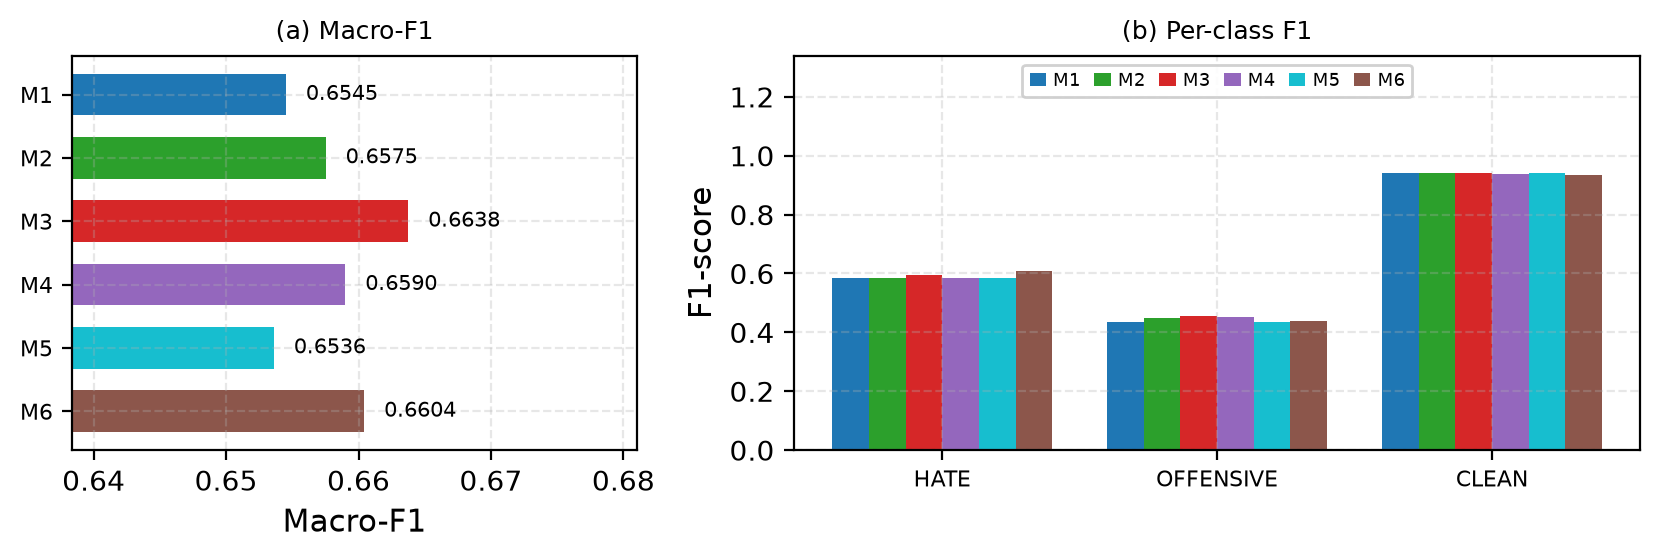
\includegraphics[width=\linewidth]{figures/comparison/f1_summary_all_models.png}\caption{\label{fig:supp-f1-summary}Macro-F1, weighted-F1 and per-class F1 side by side for every system.}\end{minipage}
\end{figure}

\begin{figure}[htbp]
\centering
\begin{minipage}{0.74\textwidth}\centering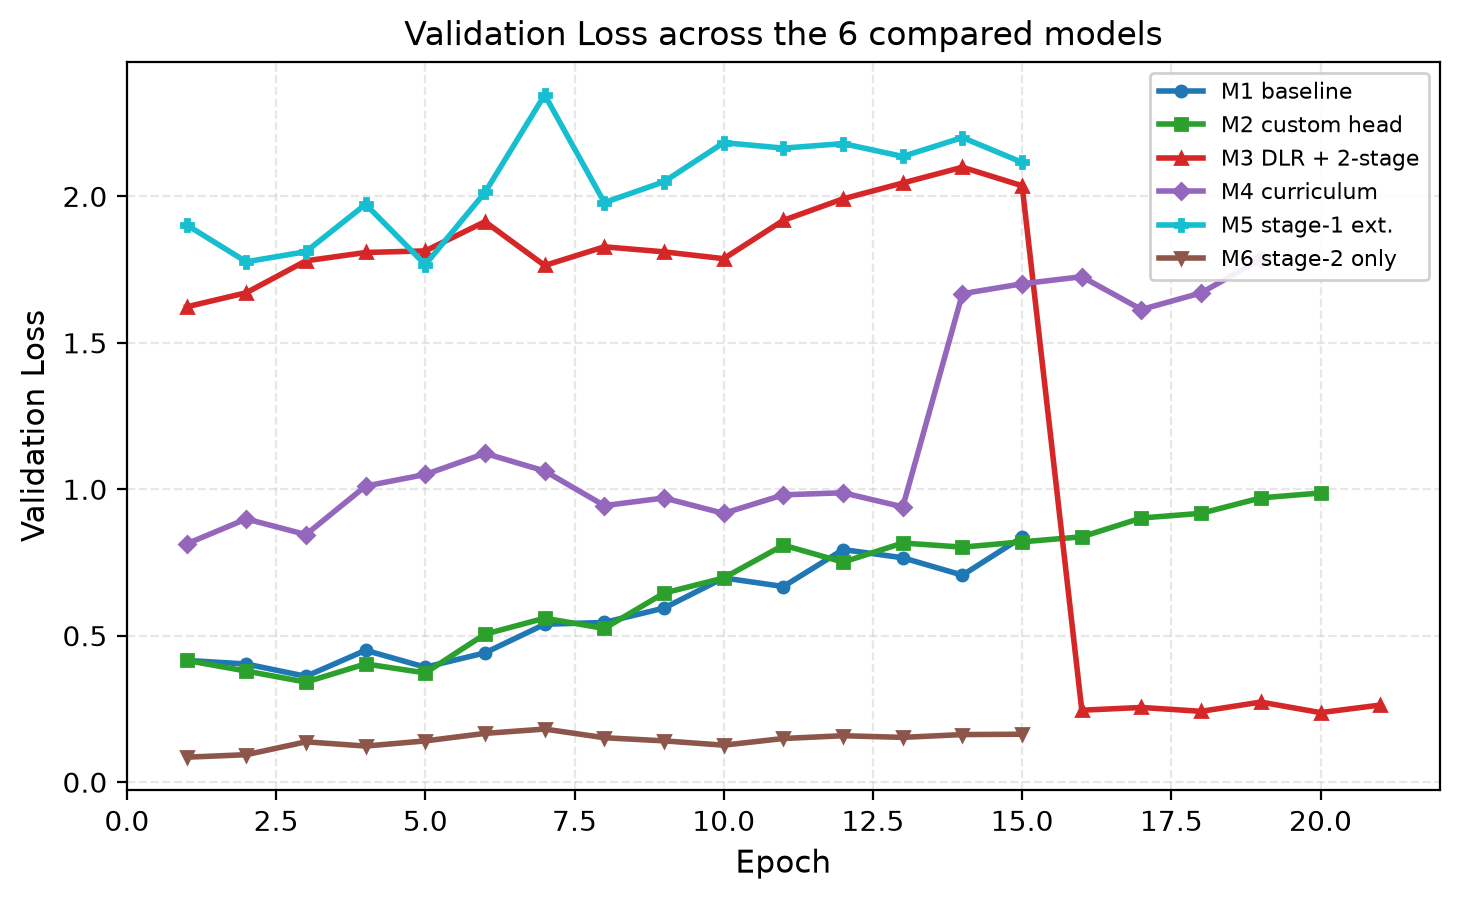
\includegraphics[width=\linewidth]{figures/comparison/validation_loss_all_models.png}\caption{\label{fig:supp-val-loss}Validation loss over the training epochs for all six systems.  The checkpoint is \emph{not} selected to minimise this curve: it is the epoch with the highest validation macro-F1 (Fig.~
ef{fig:supp-val-acc}), which is why the selected checkpoints can sit on a rising-loss epoch.}\end{minipage}
\end{figure}

\begin{figure}[htbp]
\centering
\begin{minipage}{0.74\textwidth}\centering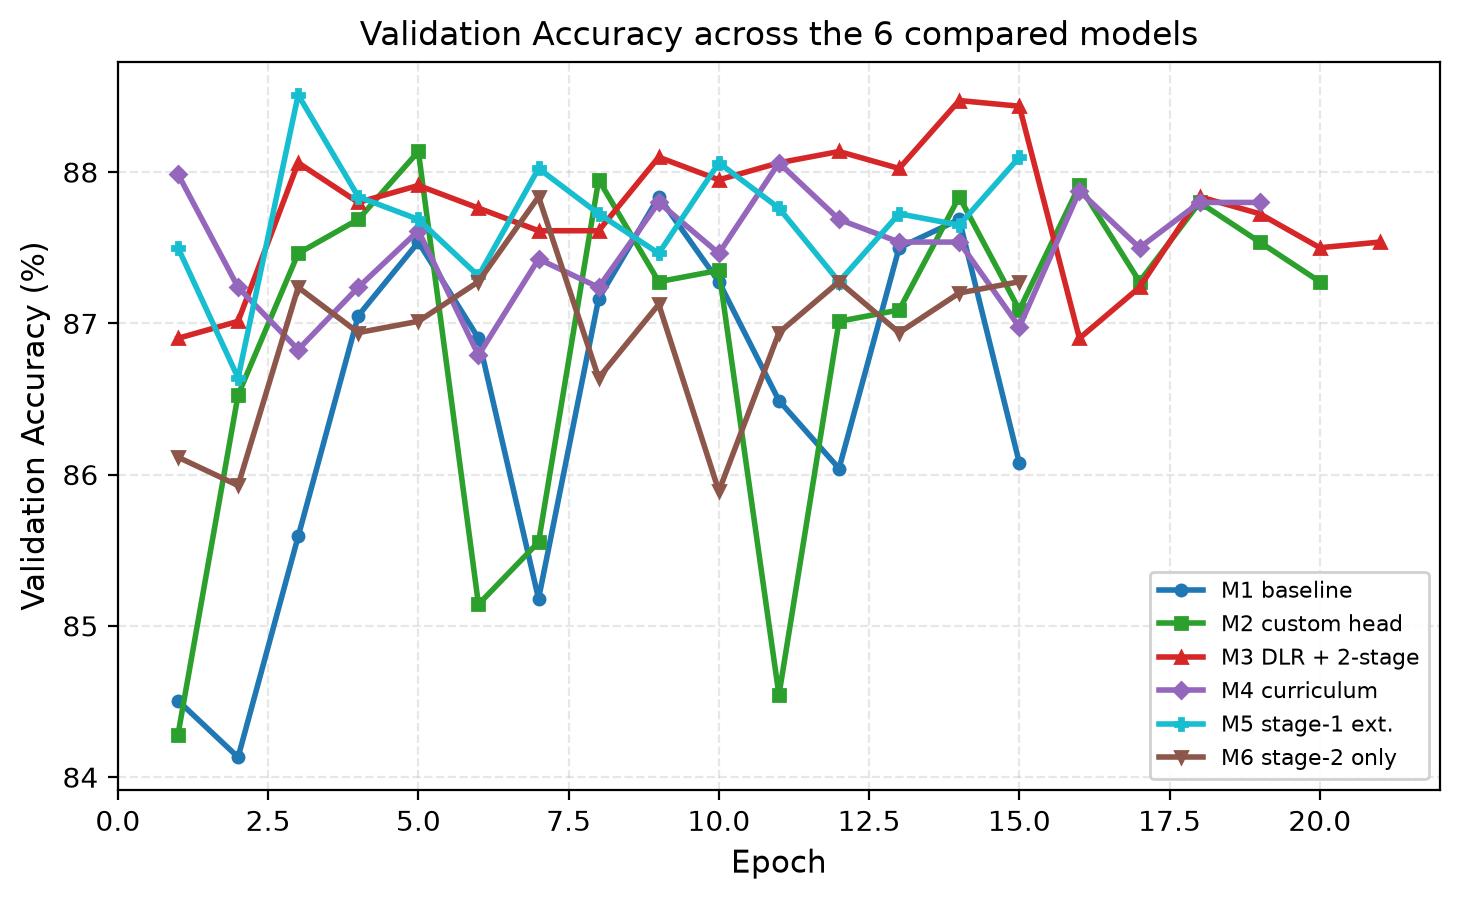
\includegraphics[width=\linewidth]{figures/comparison/validation_accuracy_all_models.png}\caption{\label{fig:supp-val-acc}Validation accuracy over the training epochs for all six systems.}\end{minipage}
\end{figure}

\begin{figure}[htbp]
\centering
\begin{minipage}{0.74\textwidth}\centering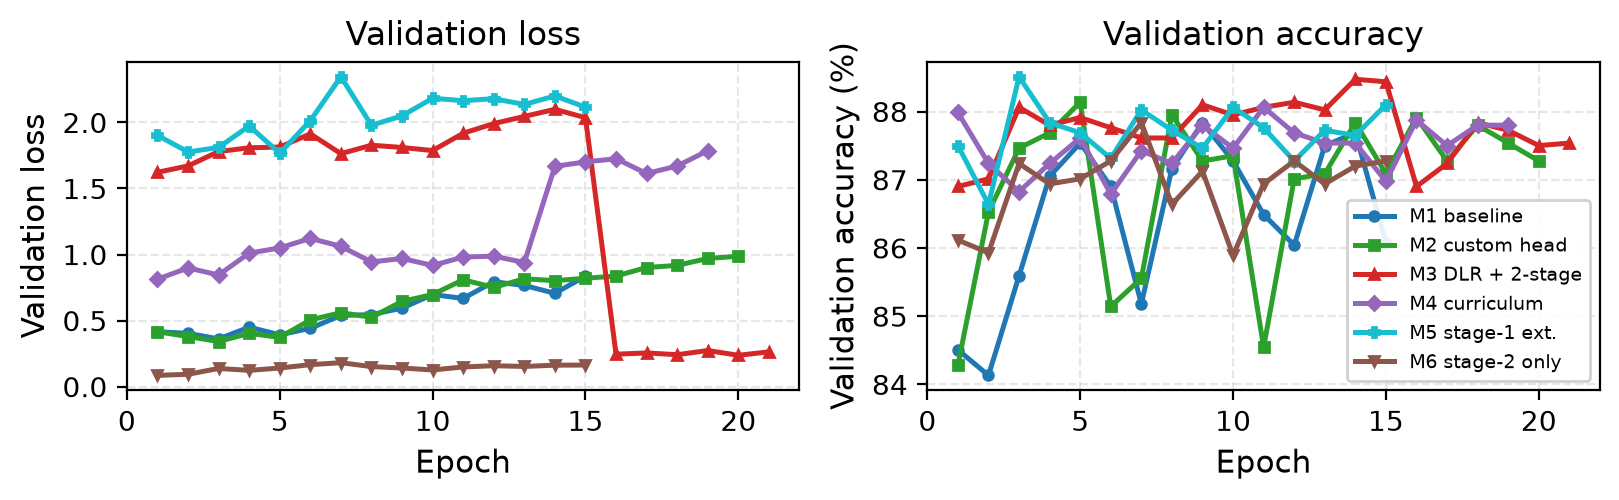
\includegraphics[width=\linewidth]{figures/comparison/validation_loss_accuracy_all_models.png}\caption{\label{fig:supp-val-loss-acc}Validation loss and accuracy on the same axes for all six systems.}\end{minipage}
\end{figure}

\begin{figure}[htbp]
\centering
\begin{minipage}{0.74\textwidth}\centering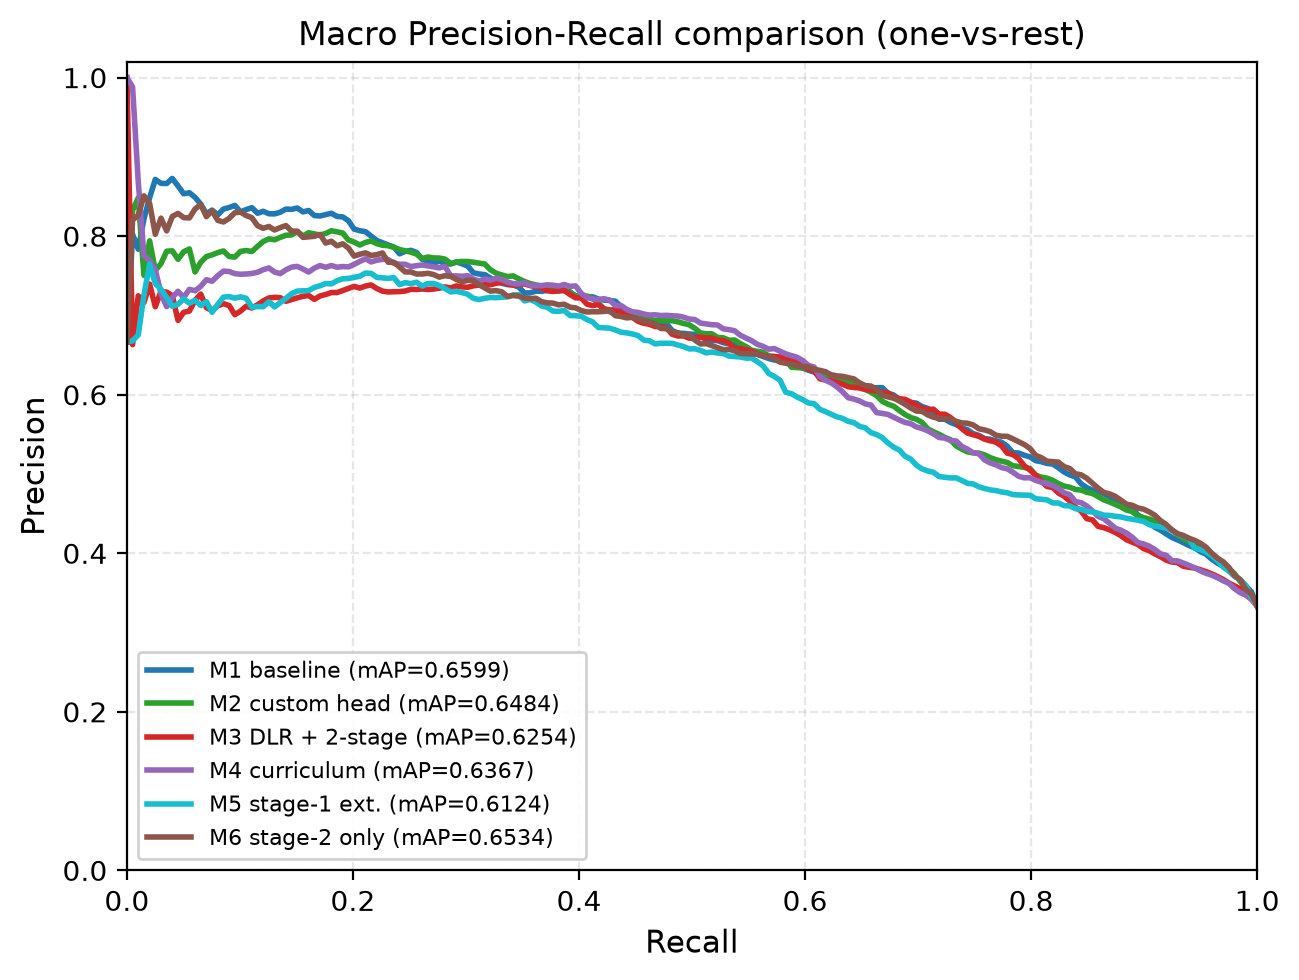
\includegraphics[width=\linewidth]{figures/comparison/pr_curve_all_models.png}\caption{\label{fig:supp-pr-all}One-vs-rest precision--recall curves (micro and macro averages) for all six systems.}\end{minipage}
\end{figure}

\begin{figure}[htbp]
\centering
\begin{minipage}{0.74\textwidth}\centering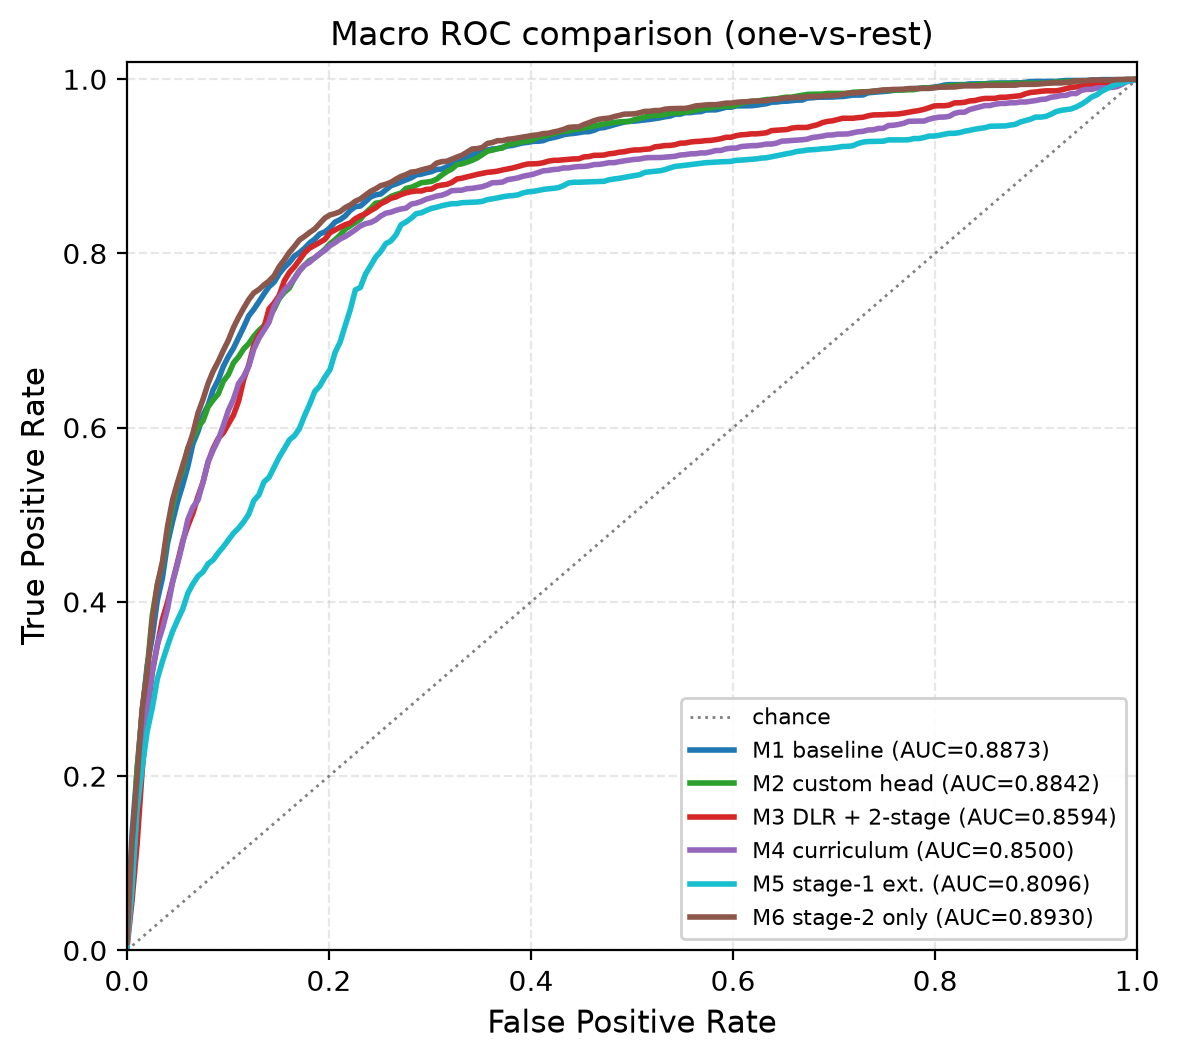
\includegraphics[width=\linewidth]{figures/comparison/roc_curve_all_models.png}\caption{\label{fig:supp-roc-all}One-vs-rest ROC curves (micro and macro averages) for all six systems.}\end{minipage}
\end{figure}

\begin{figure}[htbp]
\centering
\begin{minipage}{0.74\textwidth}\centering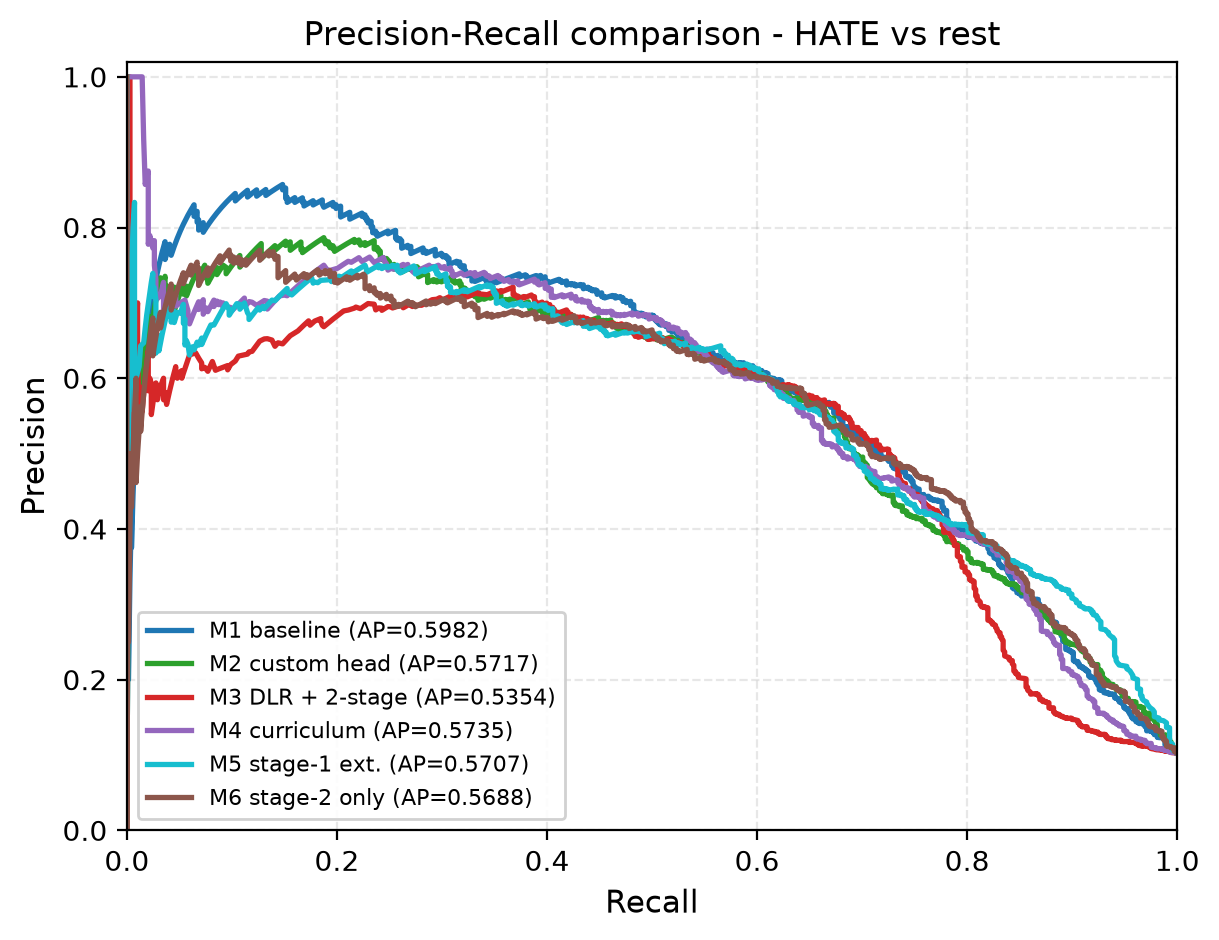
\includegraphics[width=\linewidth]{figures/comparison/pr_hate_all_models.png}\caption{\label{fig:supp-pr-hate}Precision--recall curve for the HATE class, all six systems.}\end{minipage}
\end{figure}

\begin{figure}[htbp]
\centering
\begin{minipage}{0.74\textwidth}\centering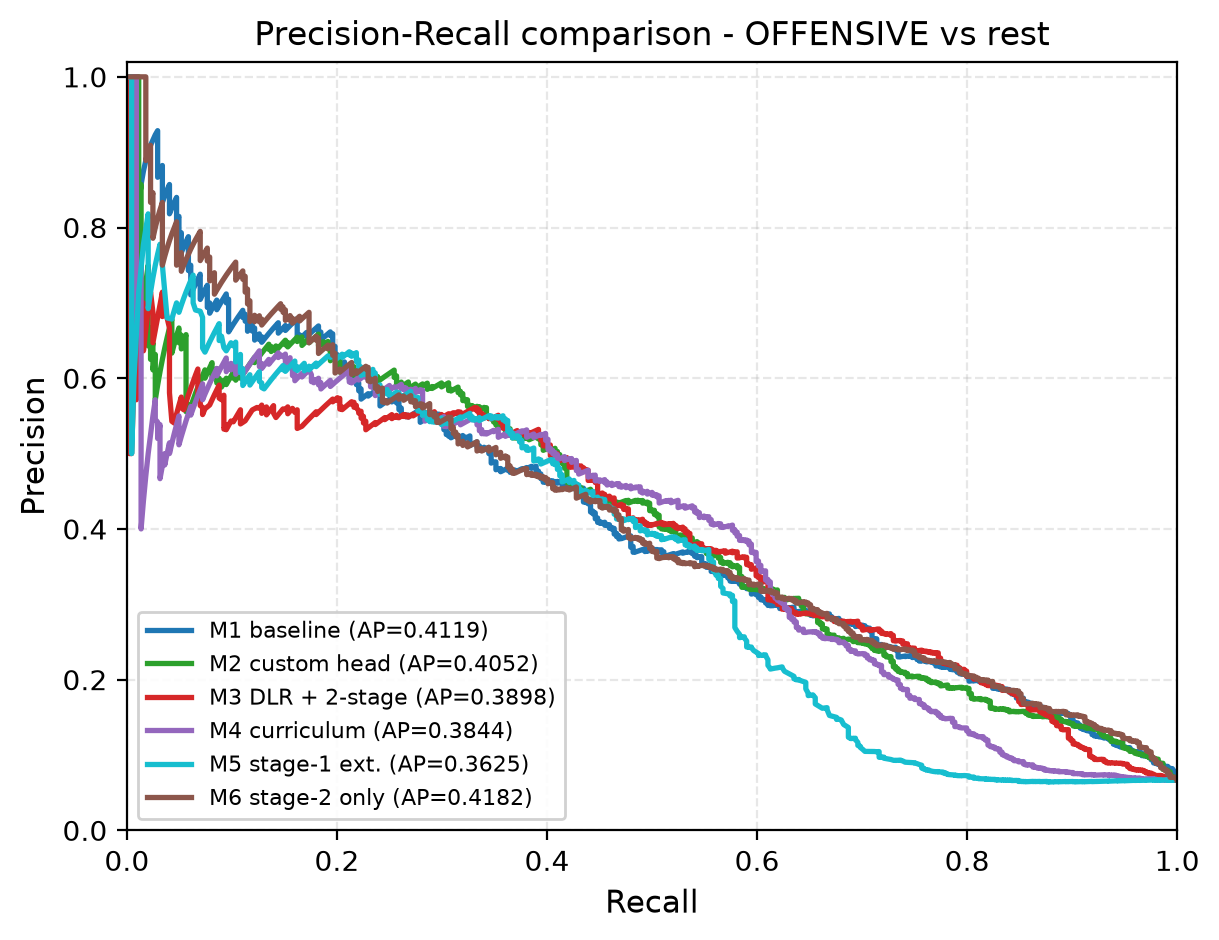
\includegraphics[width=\linewidth]{figures/comparison/pr_offensive_all_models.png}\caption{\label{fig:supp-pr-offensive}Precision--recall curve for the OFFENSIVE class, all six systems.}\end{minipage}
\end{figure}

\begin{figure}[htbp]
\centering
\begin{minipage}{0.74\textwidth}\centering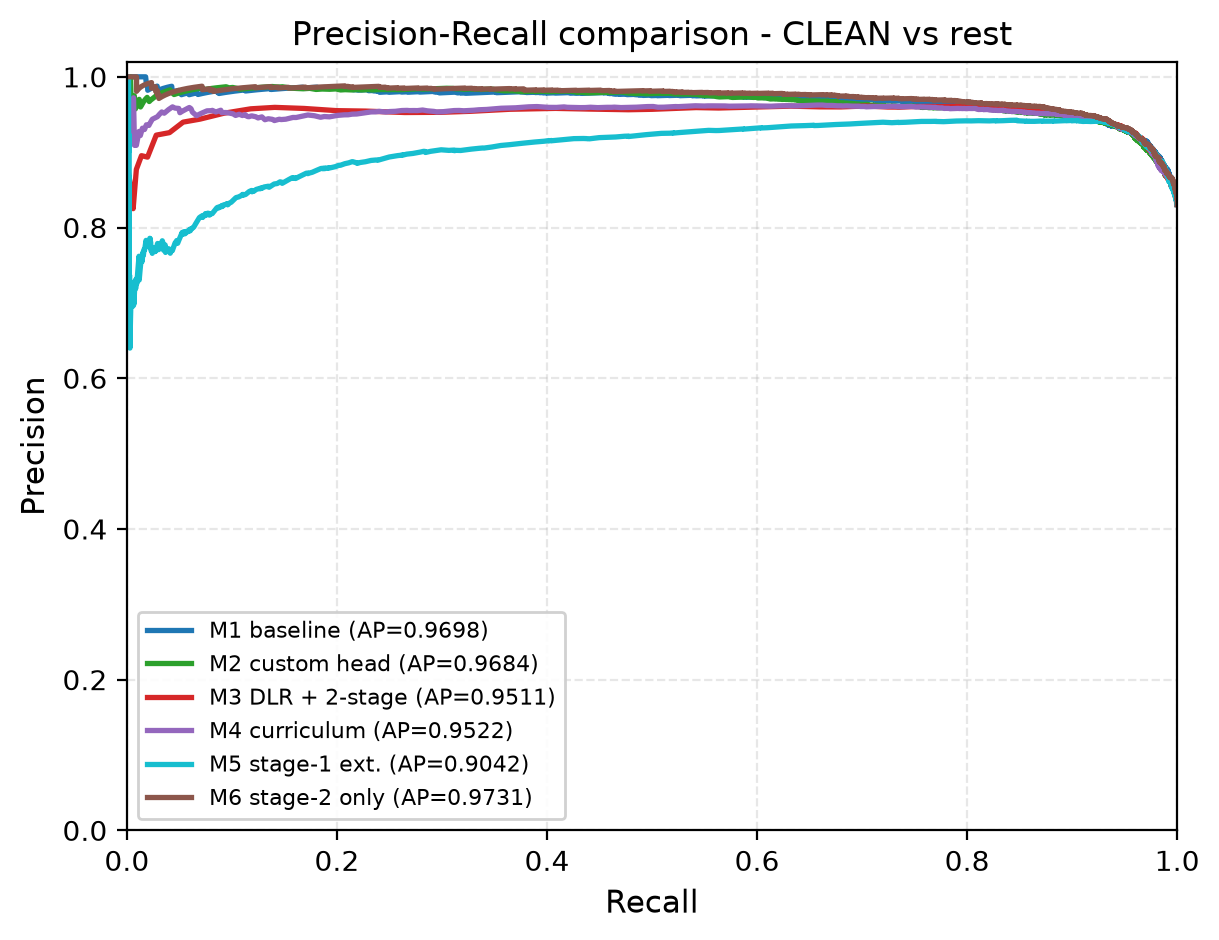
\includegraphics[width=\linewidth]{figures/comparison/pr_clean_all_models.png}\caption{\label{fig:supp-pr-clean}Precision--recall curve for the CLEAN class, all six systems.}\end{minipage}
\end{figure}

\begin{figure}[htbp]
\centering
\begin{minipage}{0.74\textwidth}\centering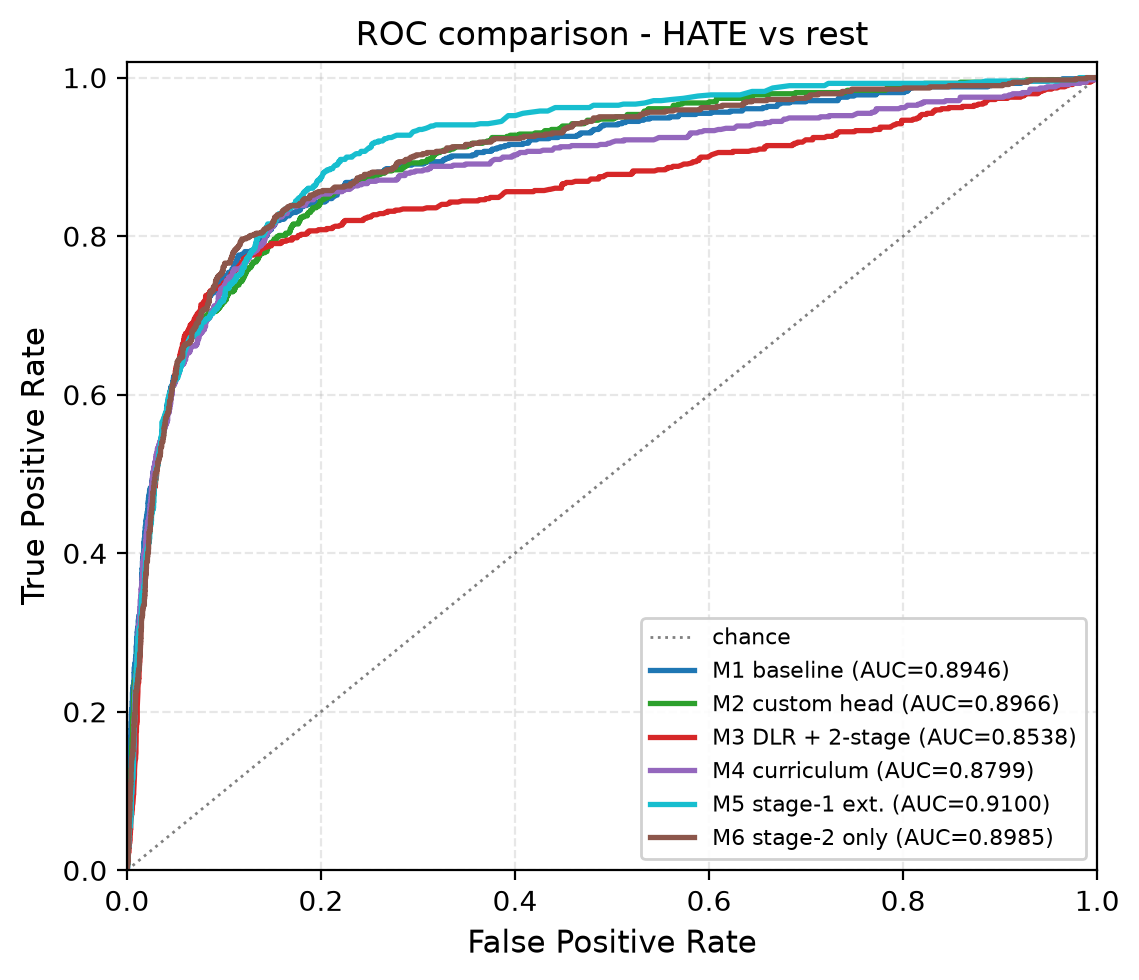
\includegraphics[width=\linewidth]{figures/comparison/roc_hate_all_models.png}\caption{\label{fig:supp-roc-hate}ROC curve for the HATE class, all six systems.}\end{minipage}
\end{figure}

\begin{figure}[htbp]
\centering
\begin{minipage}{0.74\textwidth}\centering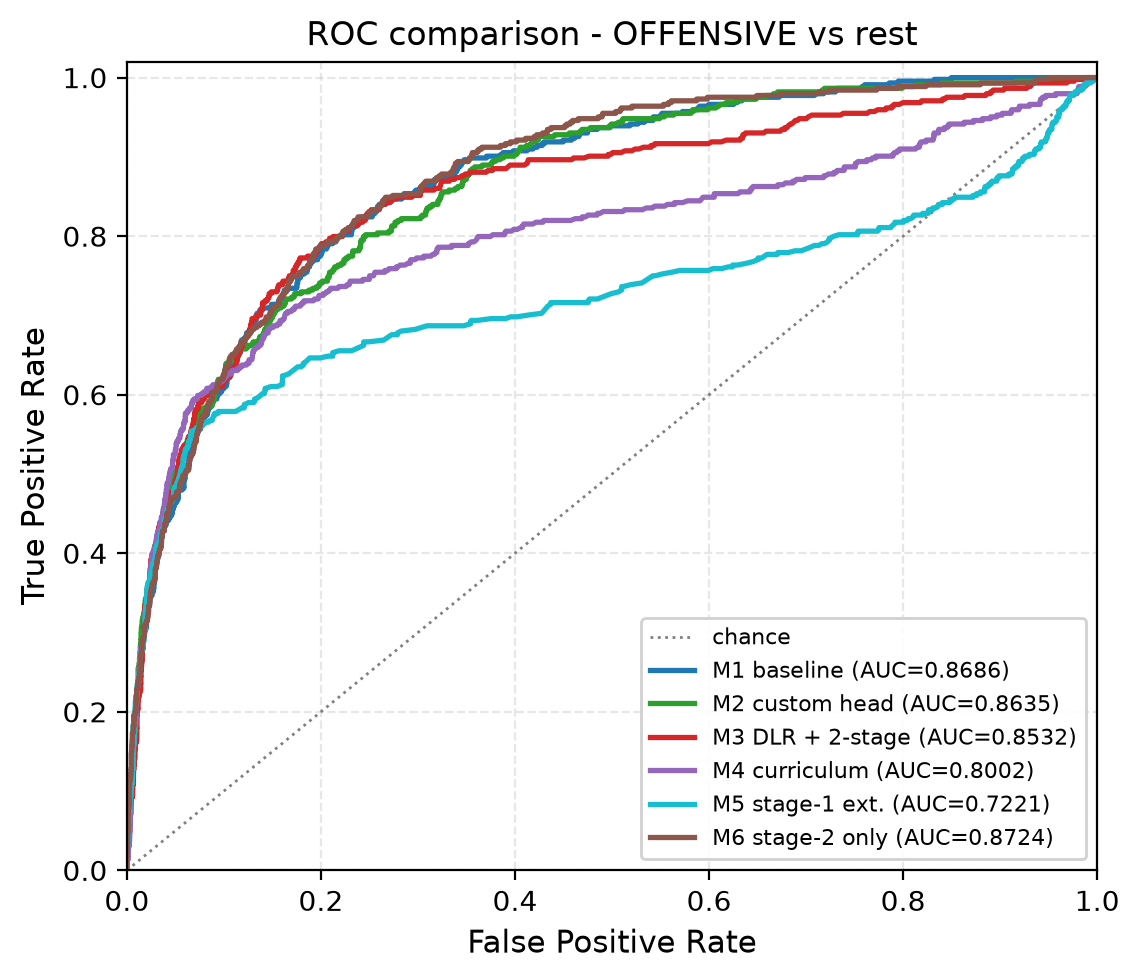
\includegraphics[width=\linewidth]{figures/comparison/roc_offensive_all_models.png}\caption{\label{fig:supp-roc-offensive}ROC curve for the OFFENSIVE class, all six systems.}\end{minipage}
\end{figure}

\begin{figure}[htbp]
\centering
\begin{minipage}{0.74\textwidth}\centering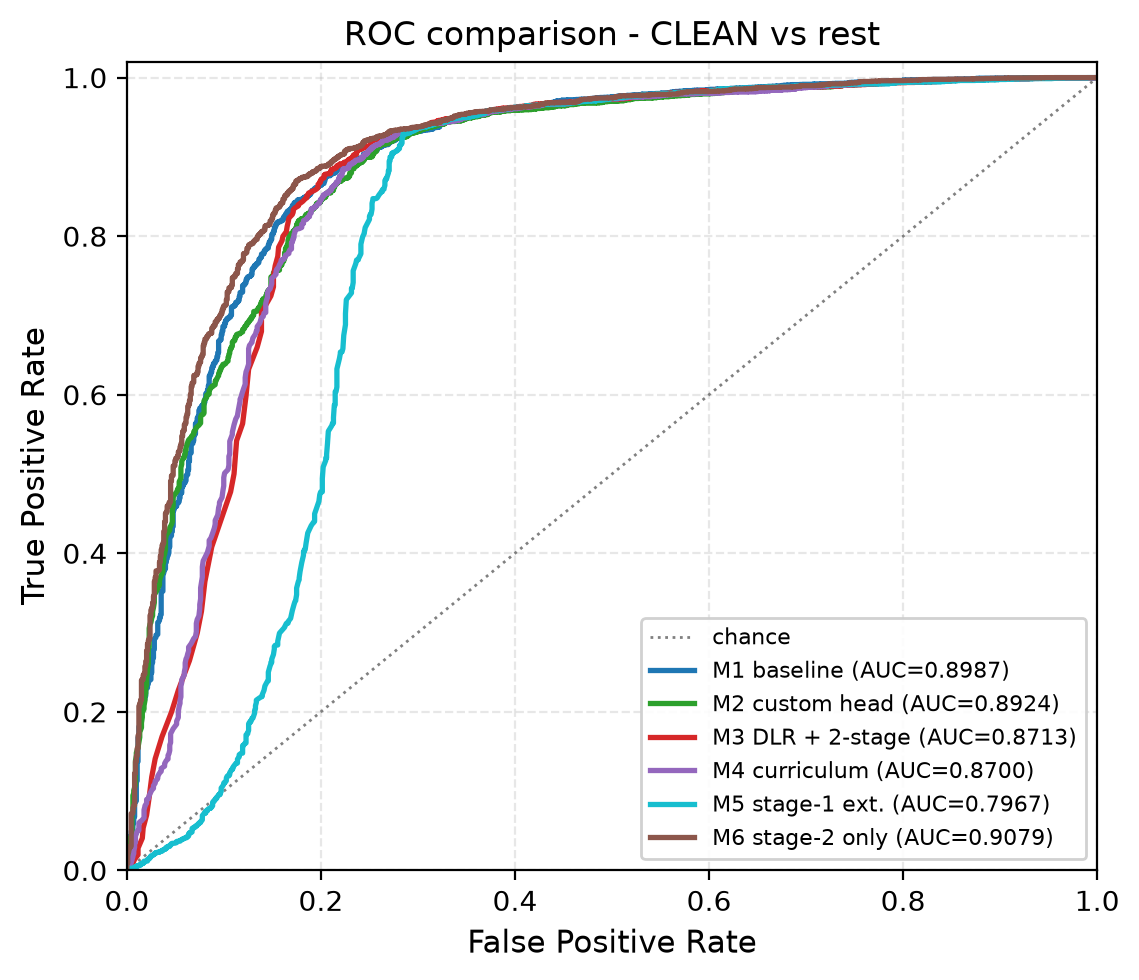
\includegraphics[width=\linewidth]{figures/comparison/roc_clean_all_models.png}\caption{\label{fig:supp-roc-clean}ROC curve for the CLEAN class, all six systems.}\end{minipage}
\end{figure}

\FloatBarrier
